\documentclass[twoside]{book}

% Packages required by doxygen
\usepackage{calc}
\usepackage{doxygen}
\usepackage{graphicx}
\usepackage[utf8]{inputenc}
\usepackage{makeidx}
\usepackage{multicol}
\usepackage{multirow}
\usepackage{textcomp}
\usepackage[table]{xcolor}

% Font selection
\usepackage[T1]{fontenc}
\usepackage{mathptmx}
\usepackage[scaled=.90]{helvet}
\usepackage{courier}
\usepackage{amssymb}
\usepackage{sectsty}
\renewcommand{\familydefault}{\sfdefault}
\allsectionsfont{%
  \fontseries{bc}\selectfont%
  \color{darkgray}%
}
\renewcommand{\DoxyLabelFont}{%
  \fontseries{bc}\selectfont%
  \color{darkgray}%
}

% Page & text layout
\usepackage{geometry}
\geometry{%
  a4paper,%
  top=2.5cm,%
  bottom=2.5cm,%
  left=2.5cm,%
  right=2.5cm%
}
\tolerance=750
\hfuzz=15pt
\hbadness=750
\setlength{\emergencystretch}{15pt}
\setlength{\parindent}{0cm}
\setlength{\parskip}{0.2cm}
\makeatletter
\renewcommand{\paragraph}{%
  \@startsection{paragraph}{4}{0ex}{-1.0ex}{1.0ex}{%
    \normalfont\normalsize\bfseries\SS@parafont%
  }%
}
\renewcommand{\subparagraph}{%
  \@startsection{subparagraph}{5}{0ex}{-1.0ex}{1.0ex}{%
    \normalfont\normalsize\bfseries\SS@subparafont%
  }%
}
\makeatother

% Headers & footers
\usepackage{fancyhdr}
\pagestyle{fancyplain}
\fancyhead[LE]{\fancyplain{}{\bfseries\thepage}}
\fancyhead[CE]{\fancyplain{}{}}
\fancyhead[RE]{\fancyplain{}{\bfseries\leftmark}}
\fancyhead[LO]{\fancyplain{}{\bfseries\rightmark}}
\fancyhead[CO]{\fancyplain{}{}}
\fancyhead[RO]{\fancyplain{}{\bfseries\thepage}}
\fancyfoot[LE]{\fancyplain{}{}}
\fancyfoot[CE]{\fancyplain{}{}}
\fancyfoot[RE]{\fancyplain{}{\bfseries\scriptsize Generated on Sun Mar 29 2015 15\-:50\-:26 for garbage-\/collector by Doxygen }}
\fancyfoot[LO]{\fancyplain{}{\bfseries\scriptsize Generated on Sun Mar 29 2015 15\-:50\-:26 for garbage-\/collector by Doxygen }}
\fancyfoot[CO]{\fancyplain{}{}}
\fancyfoot[RO]{\fancyplain{}{}}
\renewcommand{\footrulewidth}{0.4pt}
\renewcommand{\chaptermark}[1]{%
  \markboth{#1}{}%
}
\renewcommand{\sectionmark}[1]{%
  \markright{\thesection\ #1}%
}

% Indices & bibliography
\usepackage{natbib}
\usepackage[titles]{tocloft}
\setcounter{tocdepth}{3}
\setcounter{secnumdepth}{5}
\makeindex

% Hyperlinks (required, but should be loaded last)
\usepackage{ifpdf}
\ifpdf
  \usepackage[pdftex,pagebackref=true]{hyperref}
\else
  \usepackage[ps2pdf,pagebackref=true]{hyperref}
\fi
\hypersetup{%
  colorlinks=true,%
  linkcolor=blue,%
  citecolor=blue,%
  unicode%
}

% Custom commands
\newcommand{\clearemptydoublepage}{%
  \newpage{\pagestyle{empty}\cleardoublepage}%
}


%===== C O N T E N T S =====

\begin{document}

% Titlepage & ToC
\hypersetup{pageanchor=false}
\pagenumbering{roman}
\begin{titlepage}
\vspace*{7cm}
\begin{center}%
{\Large garbage-\/collector }\\
\vspace*{1cm}
{\large Generated by Doxygen 1.8.6}\\
\vspace*{0.5cm}
{\small Sun Mar 29 2015 15:50:26}\\
\end{center}
\end{titlepage}
\clearemptydoublepage
\tableofcontents
\clearemptydoublepage
\pagenumbering{arabic}
\hypersetup{pageanchor=true}

%--- Begin generated contents ---
\chapter{Hierarchical Index}
\section{Class Hierarchy}
This inheritance list is sorted roughly, but not completely, alphabetically\-:\begin{DoxyCompactList}
\item \contentsline{section}{C\-C}{\pageref{struct_c_c}}{}
\item \contentsline{section}{garbage\-\_\-collector}{\pageref{classgarbage__collector}}{}
\item \contentsline{section}{generique\-\_\-pointer}{\pageref{classgenerique__pointer}}{}
\begin{DoxyCompactList}
\item \contentsline{section}{smart\-\_\-ptr$<$ T $>$}{\pageref{classsmart__ptr}}{}
\item \contentsline{section}{smart\-\_\-ptr$<$ test\-\_\-obj $>$}{\pageref{classsmart__ptr}}{}
\end{DoxyCompactList}
\item \contentsline{section}{S\-\_\-info\-\_\-mem}{\pageref{struct_s__info__mem}}{}
\item \contentsline{section}{S\-\_\-tarjan\-\_\-info}{\pageref{struct_s__tarjan__info}}{}
\item \contentsline{section}{test\-\_\-obj}{\pageref{classtest__obj}}{}
\end{DoxyCompactList}

\chapter{Class Index}
\section{Class List}
Here are the classes, structs, unions and interfaces with brief descriptions\-:\begin{DoxyCompactList}
\item\contentsline{section}{\hyperlink{struct_c_c}{C\-C} }{\pageref{struct_c_c}}{}
\item\contentsline{section}{\hyperlink{classgarbage__collector}{garbage\-\_\-collector} \\*This class represent our garbage collector }{\pageref{classgarbage__collector}}{}
\item\contentsline{section}{\hyperlink{classgenerique__pointer}{generique\-\_\-pointer} \\*General behavior of a smart pointer }{\pageref{classgenerique__pointer}}{}
\item\contentsline{section}{\hyperlink{struct_s__info__mem}{S\-\_\-info\-\_\-mem} }{\pageref{struct_s__info__mem}}{}
\item\contentsline{section}{\hyperlink{struct_s__tarjan__info}{S\-\_\-tarjan\-\_\-info} }{\pageref{struct_s__tarjan__info}}{}
\item\contentsline{section}{\hyperlink{classsmart__ptr}{smart\-\_\-ptr$<$ T $>$} \\*Our Smart pointer implementation }{\pageref{classsmart__ptr}}{}
\item\contentsline{section}{\hyperlink{classtest__obj}{test\-\_\-obj} \\*Just a testing class to ensure the behavior of our smartpointers and G\-C }{\pageref{classtest__obj}}{}
\end{DoxyCompactList}

\chapter{Class Documentation}
\hypertarget{struct_c_c}{\section{C\-C Struct Reference}
\label{struct_c_c}\index{C\-C@{C\-C}}
}
\subsection*{Public Member Functions}
\begin{DoxyCompactItemize}
\item 
\hypertarget{struct_c_c_a44f3e83081f562b68aec02302ad13e91}{{\bfseries P\-O\-I\-N\-T\-E\-U\-R} (\hyperlink{struct_c_c}{C\-C}) p}\label{struct_c_c_a44f3e83081f562b68aec02302ad13e91}

\end{DoxyCompactItemize}


The documentation for this struct was generated from the following file\-:\begin{DoxyCompactItemize}
\item 
src/main.\-cpp\end{DoxyCompactItemize}

\hypertarget{classgarbage__collector}{\section{garbage\-\_\-collector Class Reference}
\label{classgarbage__collector}\index{garbage\-\_\-collector@{garbage\-\_\-collector}}
}


This class represent our garbage collector.  




{\ttfamily \#include $<$garbage\-\_\-collector.\-hpp$>$}

\subsection*{Public Member Functions}
\begin{DoxyCompactItemize}
\item 
void \hyperlink{classgarbage__collector_a09aba23f6c605cad9b8d06a68d1ccb3d}{on\-\_\-attach} (void $\ast$mem, \hyperlink{classgenerique__pointer}{generique\-\_\-pointer} \&ptr)
\begin{DoxyCompactList}\small\item\em Register an association smart\-\_\-pointer to memoryblock on the garbage collector. \end{DoxyCompactList}\item 
{\footnotesize template$<$typename T $>$ }\\void \hyperlink{classgarbage__collector_a03cb5dbdb08bbbb52a116b2499905fd2}{on\-\_\-detach} (void $\ast$mem, \hyperlink{classgenerique__pointer}{generique\-\_\-pointer} \&ptr)
\begin{DoxyCompactList}\small\item\em Unregister an association smart\-\_\-pointer to memoryblock to the garbage collector. \end{DoxyCompactList}\item 
void \hyperlink{classgarbage__collector_a7819a3496e0090520bcf8504f8a1fa6e}{on\-\_\-new} (void $\ast$memblock, std\-::size\-\_\-t size)
\begin{DoxyCompactList}\small\item\em Notify the garbage collector of a new allocated blocks. \end{DoxyCompactList}\end{DoxyCompactItemize}
\subsection*{Static Public Member Functions}
\begin{DoxyCompactItemize}
\item 
\hypertarget{classgarbage__collector_a006a84658a8b06f5f0adf151b9909edc}{static \hyperlink{classgarbage__collector}{garbage\-\_\-collector} \& \hyperlink{classgarbage__collector_a006a84658a8b06f5f0adf151b9909edc}{get\-\_\-instance} ()}\label{classgarbage__collector_a006a84658a8b06f5f0adf151b9909edc}

\begin{DoxyCompactList}\small\item\em Get the instance of the singleton. \end{DoxyCompactList}\end{DoxyCompactItemize}


\subsection{Detailed Description}
This class represent our garbage collector. 

\subsection{Member Function Documentation}
\hypertarget{classgarbage__collector_a09aba23f6c605cad9b8d06a68d1ccb3d}{\index{garbage\-\_\-collector@{garbage\-\_\-collector}!on\-\_\-attach@{on\-\_\-attach}}
\index{on\-\_\-attach@{on\-\_\-attach}!garbage_collector@{garbage\-\_\-collector}}
\subsubsection[{on\-\_\-attach}]{\setlength{\rightskip}{0pt plus 5cm}void garbage\-\_\-collector\-::on\-\_\-attach (
\begin{DoxyParamCaption}
\item[{void $\ast$}]{mem, }
\item[{{\bf generique\-\_\-pointer} \&}]{ptr}
\end{DoxyParamCaption}
)}}\label{classgarbage__collector_a09aba23f6c605cad9b8d06a68d1ccb3d}


Register an association smart\-\_\-pointer to memoryblock on the garbage collector. 


\begin{DoxyParams}{Parameters}
{\em mem} & the memory block used by the smartpointer \\
\hline
{\em ptr} & the smartpointer \\
\hline
\end{DoxyParams}
\hypertarget{classgarbage__collector_a03cb5dbdb08bbbb52a116b2499905fd2}{\index{garbage\-\_\-collector@{garbage\-\_\-collector}!on\-\_\-detach@{on\-\_\-detach}}
\index{on\-\_\-detach@{on\-\_\-detach}!garbage_collector@{garbage\-\_\-collector}}
\subsubsection[{on\-\_\-detach}]{\setlength{\rightskip}{0pt plus 5cm}template$<$typename T $>$ void garbage\-\_\-collector\-::on\-\_\-detach (
\begin{DoxyParamCaption}
\item[{void $\ast$}]{mem, }
\item[{{\bf generique\-\_\-pointer} \&}]{ptr}
\end{DoxyParamCaption}
)}}\label{classgarbage__collector_a03cb5dbdb08bbbb52a116b2499905fd2}


Unregister an association smart\-\_\-pointer to memoryblock to the garbage collector. 


\begin{DoxyParams}{Parameters}
{\em mem} & \\
\hline
{\em ptr} & \\
\hline
\end{DoxyParams}
\hypertarget{classgarbage__collector_a7819a3496e0090520bcf8504f8a1fa6e}{\index{garbage\-\_\-collector@{garbage\-\_\-collector}!on\-\_\-new@{on\-\_\-new}}
\index{on\-\_\-new@{on\-\_\-new}!garbage_collector@{garbage\-\_\-collector}}
\subsubsection[{on\-\_\-new}]{\setlength{\rightskip}{0pt plus 5cm}void garbage\-\_\-collector\-::on\-\_\-new (
\begin{DoxyParamCaption}
\item[{void $\ast$}]{memblock, }
\item[{std\-::size\-\_\-t}]{size}
\end{DoxyParamCaption}
)}}\label{classgarbage__collector_a7819a3496e0090520bcf8504f8a1fa6e}


Notify the garbage collector of a new allocated blocks. 


\begin{DoxyParams}{Parameters}
{\em void} & $\ast$ the adress of the new element \\
\hline
{\em std\-::size\-\_\-t} & the size of the new block \\
\hline
\end{DoxyParams}


The documentation for this class was generated from the following files\-:\begin{DoxyCompactItemize}
\item 
src/garbage\-\_\-collector.\-hpp\item 
src/garbage\-\_\-collector.\-cpp\end{DoxyCompactItemize}

\hypertarget{classgenerique__pointer}{\section{generique\-\_\-pointer Class Reference}
\label{classgenerique__pointer}\index{generique\-\_\-pointer@{generique\-\_\-pointer}}
}


general behavior of a smart pointer  




{\ttfamily \#include $<$generique\-\_\-pointer.\-hpp$>$}

Inheritance diagram for generique\-\_\-pointer\-:\begin{figure}[H]
\begin{center}
\leavevmode
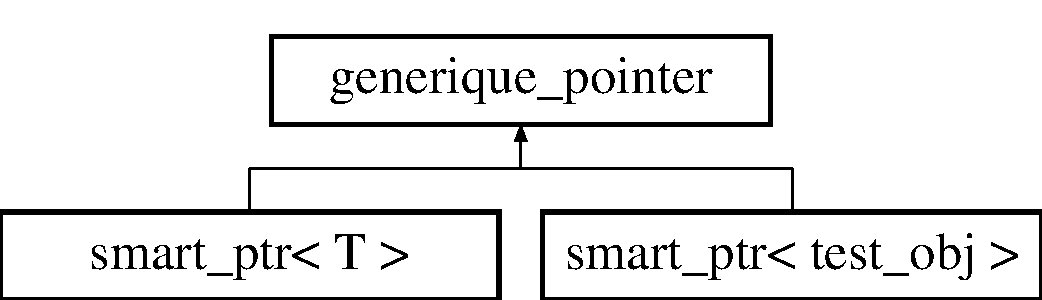
\includegraphics[height=2.000000cm]{classgenerique__pointer}
\end{center}
\end{figure}
\subsection*{Public Member Functions}
\begin{DoxyCompactItemize}
\item 
\hypertarget{classgenerique__pointer_a5b24c4b97a0cb5fcda64ea2f4c5d3453}{\hyperlink{classgenerique__pointer_a5b24c4b97a0cb5fcda64ea2f4c5d3453}{generique\-\_\-pointer} ()}\label{classgenerique__pointer_a5b24c4b97a0cb5fcda64ea2f4c5d3453}

\begin{DoxyCompactList}\small\item\em default constructor \end{DoxyCompactList}\item 
\hypertarget{classgenerique__pointer_ae4baa1231b8dae1c6b91e797e1f91f20}{virtual \hyperlink{classgenerique__pointer_ae4baa1231b8dae1c6b91e797e1f91f20}{$\sim$generique\-\_\-pointer} ()}\label{classgenerique__pointer_ae4baa1231b8dae1c6b91e797e1f91f20}

\begin{DoxyCompactList}\small\item\em destructor \end{DoxyCompactList}\item 
\hypertarget{classgenerique__pointer_aba1453e54c31ec0c1a7eb3ff39d524e0}{virtual void \hyperlink{classgenerique__pointer_aba1453e54c31ec0c1a7eb3ff39d524e0}{force\-\_\-detach} ()=0}\label{classgenerique__pointer_aba1453e54c31ec0c1a7eb3ff39d524e0}

\begin{DoxyCompactList}\small\item\em virtual fonction, implemented in \hyperlink{smart__ptr_8hpp_source}{smart\-\_\-ptr.\-hpp} \end{DoxyCompactList}\item 
\hypertarget{classgenerique__pointer_ac8b533fc0ae3940063a292000b63dbe9}{virtual void $\ast$ \hyperlink{classgenerique__pointer_ac8b533fc0ae3940063a292000b63dbe9}{get\-\_\-addr} () const =0}\label{classgenerique__pointer_ac8b533fc0ae3940063a292000b63dbe9}

\begin{DoxyCompactList}\small\item\em virtual fonction, implemented in \hyperlink{smart__ptr_8hpp_source}{smart\-\_\-ptr.\-hpp} \end{DoxyCompactList}\item 
\hypertarget{classgenerique__pointer_aa3deb91c80435eff11436d790cd7445a}{bool \hyperlink{classgenerique__pointer_aa3deb91c80435eff11436d790cd7445a}{operator==} (const \hyperlink{classgenerique__pointer}{generique\-\_\-pointer} \&rhs) const }\label{classgenerique__pointer_aa3deb91c80435eff11436d790cd7445a}

\begin{DoxyCompactList}\small\item\em return egality on generics pointers on their id attribute \end{DoxyCompactList}\item 
bool \hyperlink{classgenerique__pointer_aa0bb852a9dd5f12769932871411dcf51}{operator$<$} (const \hyperlink{classgenerique__pointer}{generique\-\_\-pointer} \&rhs) const 
\begin{DoxyCompactList}\small\item\em compare two generics pointers on their id attributes \end{DoxyCompactList}\end{DoxyCompactItemize}
\subsection*{Static Public Member Functions}
\begin{DoxyCompactItemize}
\item 
\hypertarget{classgenerique__pointer_aaf4a48370e6f36530d7e1f7a9ee8e376}{static long \hyperlink{classgenerique__pointer_aaf4a48370e6f36530d7e1f7a9ee8e376}{inc\-\_\-compteur} ()}\label{classgenerique__pointer_aaf4a48370e6f36530d7e1f7a9ee8e376}

\begin{DoxyCompactList}\small\item\em increment a variable to count and identify all pointers \end{DoxyCompactList}\end{DoxyCompactItemize}


\subsection{Detailed Description}
general behavior of a smart pointer 

\subsection{Member Function Documentation}
\hypertarget{classgenerique__pointer_aa0bb852a9dd5f12769932871411dcf51}{\index{generique\-\_\-pointer@{generique\-\_\-pointer}!operator$<$@{operator$<$}}
\index{operator$<$@{operator$<$}!generique_pointer@{generique\-\_\-pointer}}
\subsubsection[{operator$<$}]{\setlength{\rightskip}{0pt plus 5cm}bool generique\-\_\-pointer\-::operator$<$ (
\begin{DoxyParamCaption}
\item[{const {\bf generique\-\_\-pointer} \&}]{rhs}
\end{DoxyParamCaption}
) const\hspace{0.3cm}{\ttfamily [inline]}}}\label{classgenerique__pointer_aa0bb852a9dd5f12769932871411dcf51}


compare two generics pointers on their id attributes 



The documentation for this class was generated from the following files\-:\begin{DoxyCompactItemize}
\item 
src/generique\-\_\-pointer.\-hpp\item 
src/generique\-\_\-pointer.\-cpp\end{DoxyCompactItemize}

\hypertarget{struct_s__info__mem}{\section{S\-\_\-info\-\_\-mem Struct Reference}
\label{struct_s__info__mem}\index{S\-\_\-info\-\_\-mem@{S\-\_\-info\-\_\-mem}}
}
\subsection*{Public Attributes}
\begin{DoxyCompactItemize}
\item 
\hypertarget{struct_s__info__mem_ade17a89d93e762516b2a2ed4ae292a9d}{std\-::set$<$ \hyperlink{classgenerique__pointer}{generique\-\_\-pointer} $\ast$ $>$ {\bfseries in}}\label{struct_s__info__mem_ade17a89d93e762516b2a2ed4ae292a9d}

\item 
\hypertarget{struct_s__info__mem_ab323a942560d3e543bbce86da40fd083}{std\-::set$<$ \hyperlink{classgenerique__pointer}{generique\-\_\-pointer} $\ast$ $>$ {\bfseries out}}\label{struct_s__info__mem_ab323a942560d3e543bbce86da40fd083}

\item 
\hypertarget{struct_s__info__mem_a868968165ef01c123473007b3c654ceb}{std\-::size\-\_\-t {\bfseries size}}\label{struct_s__info__mem_a868968165ef01c123473007b3c654ceb}

\item 
\hypertarget{struct_s__info__mem_a2eb61729e6efa09a23957a7dcca0f667}{bool {\bfseries valid}}\label{struct_s__info__mem_a2eb61729e6efa09a23957a7dcca0f667}

\end{DoxyCompactItemize}


The documentation for this struct was generated from the following file\-:\begin{DoxyCompactItemize}
\item 
src/garbage\-\_\-collector.\-hpp\end{DoxyCompactItemize}

\hypertarget{struct_s__tarjan__info}{\section{S\-\_\-tarjan\-\_\-info Struct Reference}
\label{struct_s__tarjan__info}\index{S\-\_\-tarjan\-\_\-info@{S\-\_\-tarjan\-\_\-info}}
}
\subsection*{Public Attributes}
\begin{DoxyCompactItemize}
\item 
\hypertarget{struct_s__tarjan__info_a054e1b778032beb34b3f9edd521c3c9d}{unsigned int {\bfseries index}}\label{struct_s__tarjan__info_a054e1b778032beb34b3f9edd521c3c9d}

\item 
\hypertarget{struct_s__tarjan__info_a59d2913d1d63aefdeaa855805b7c6e15}{unsigned int {\bfseries lowlink}}\label{struct_s__tarjan__info_a59d2913d1d63aefdeaa855805b7c6e15}

\item 
\hypertarget{struct_s__tarjan__info_a9a78c59b92d785199271341da32acb92}{bool {\bfseries on\-Stack}}\label{struct_s__tarjan__info_a9a78c59b92d785199271341da32acb92}

\end{DoxyCompactItemize}


The documentation for this struct was generated from the following file\-:\begin{DoxyCompactItemize}
\item 
src/garbage\-\_\-collector.\-hpp\end{DoxyCompactItemize}

\hypertarget{classsmart__ptr}{\section{smart\-\_\-ptr$<$ T $>$ Class Template Reference}
\label{classsmart__ptr}\index{smart\-\_\-ptr$<$ T $>$@{smart\-\_\-ptr$<$ T $>$}}
}


Our Smart pointer implementation.  




{\ttfamily \#include $<$smart\-\_\-ptr.\-hpp$>$}

Inheritance diagram for smart\-\_\-ptr$<$ T $>$\-:\begin{figure}[H]
\begin{center}
\leavevmode
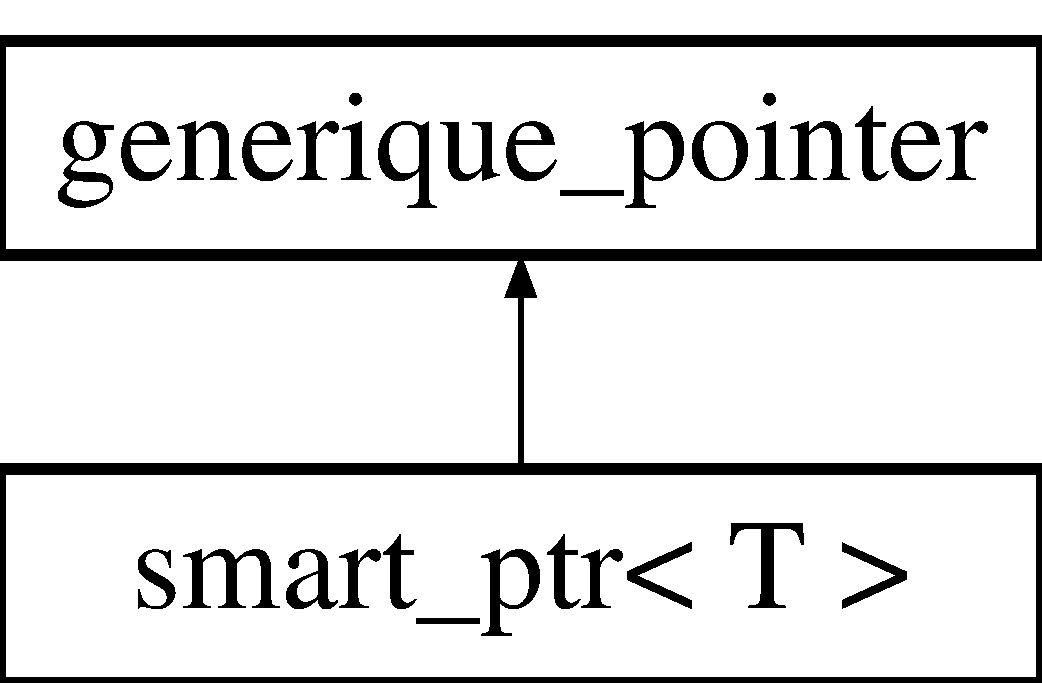
\includegraphics[height=2.000000cm]{classsmart__ptr}
\end{center}
\end{figure}
\subsection*{Public Member Functions}
\begin{DoxyCompactItemize}
\item 
\hypertarget{classsmart__ptr_ae09faa6aeb5dd0f9587174c279410c4c}{\hyperlink{classsmart__ptr_ae09faa6aeb5dd0f9587174c279410c4c}{smart\-\_\-ptr} ()}\label{classsmart__ptr_ae09faa6aeb5dd0f9587174c279410c4c}

\begin{DoxyCompactList}\small\item\em Construct a new smartpointer pointing to N\-U\-L\-L. \end{DoxyCompactList}\item 
\hyperlink{classsmart__ptr_a9a21ea7b2a253280c101b85b31ad2074}{smart\-\_\-ptr} (const \hyperlink{classsmart__ptr}{smart\-\_\-ptr} \&rhs)
\item 
\hyperlink{classsmart__ptr_aa2d4a2bcc8befc68a31d340d97b3b33c}{smart\-\_\-ptr} (T $\ast$var\-\_\-elem)
\item 
\hyperlink{classsmart__ptr_a43518f1c6d475b5d462599780f07b769}{$\sim$smart\-\_\-ptr} ()
\begin{DoxyCompactList}\small\item\em Destruct the Smart\-Pointer, and notify the garbage collector. \end{DoxyCompactList}\item 
\hypertarget{classsmart__ptr_abc00d30772eeb6050f2db0639a80eb5f}{\hyperlink{classsmart__ptr}{smart\-\_\-ptr}$<$ T $>$ \& \hyperlink{classsmart__ptr_abc00d30772eeb6050f2db0639a80eb5f}{operator=} (T $\ast$var\-\_\-elem)}\label{classsmart__ptr_abc00d30772eeb6050f2db0639a80eb5f}

\begin{DoxyCompactList}\small\item\em Overload of operator = in case of accessing to element. \end{DoxyCompactList}\item 
\hypertarget{classsmart__ptr_abf4c44d2c4b0ded71dfa05ded4da6319}{\hyperlink{classsmart__ptr}{smart\-\_\-ptr}$<$ T $>$ \& \hyperlink{classsmart__ptr_abf4c44d2c4b0ded71dfa05ded4da6319}{operator=} (const \hyperlink{classsmart__ptr}{smart\-\_\-ptr}$<$ T $>$ \&ptr)}\label{classsmart__ptr_abf4c44d2c4b0ded71dfa05ded4da6319}

\begin{DoxyCompactList}\small\item\em overload operator = in case of affectation to another smart pointers \end{DoxyCompactList}\item 
\hypertarget{classsmart__ptr_ad7e692635bc33199ee7304d70279852b}{\hyperlink{classsmart__ptr}{smart\-\_\-ptr}$<$ T $>$ \& \hyperlink{classsmart__ptr_ad7e692635bc33199ee7304d70279852b}{operator=} (void $\ast$var\-\_\-elem)}\label{classsmart__ptr_ad7e692635bc33199ee7304d70279852b}

\begin{DoxyCompactList}\small\item\em overload operator = in case of affectation to a generic adress \end{DoxyCompactList}\item 
\hypertarget{classsmart__ptr_ae9512b5bbf3d31ea4d72d9f53b4f9aae}{virtual T \& \hyperlink{classsmart__ptr_ae9512b5bbf3d31ea4d72d9f53b4f9aae}{operator$\ast$} () const }\label{classsmart__ptr_ae9512b5bbf3d31ea4d72d9f53b4f9aae}

\begin{DoxyCompactList}\small\item\em Deferencing element to access element. \end{DoxyCompactList}\item 
\hypertarget{classsmart__ptr_a5335c11a725ec08cf9e178a5a87c0aa0}{T $\ast$ \hyperlink{classsmart__ptr_a5335c11a725ec08cf9e178a5a87c0aa0}{operator-\/$>$} () const }\label{classsmart__ptr_a5335c11a725ec08cf9e178a5a87c0aa0}

\begin{DoxyCompactList}\small\item\em Overload arrow operator to member access on the pointed element. \end{DoxyCompactList}\item 
\hypertarget{classsmart__ptr_a56b7836a7c412867e75e95626f83576e}{bool \hyperlink{classsmart__ptr_a56b7836a7c412867e75e95626f83576e}{operator==} (const T $\ast$r\-\_\-member)}\label{classsmart__ptr_a56b7836a7c412867e75e95626f83576e}

\begin{DoxyCompactList}\small\item\em Egality operator. \end{DoxyCompactList}\item 
\hypertarget{classsmart__ptr_a381c1f77e00684276099482b02b652a7}{T \& \hyperlink{classsmart__ptr_a381c1f77e00684276099482b02b652a7}{operator\mbox{[}$\,$\mbox{]}} (std\-::size\-\_\-t idx)}\label{classsmart__ptr_a381c1f77e00684276099482b02b652a7}

\begin{DoxyCompactList}\small\item\em Overload \mbox{[}\mbox{]} operator to provide array-\/like access allowing both reading and writing. \end{DoxyCompactList}\item 
\hypertarget{classsmart__ptr_a7aa281850218c59e7c8cf12a6f934e62}{const T \& \hyperlink{classsmart__ptr_a7aa281850218c59e7c8cf12a6f934e62}{operator\mbox{[}$\,$\mbox{]}} (std\-::size\-\_\-t idx) const }\label{classsmart__ptr_a7aa281850218c59e7c8cf12a6f934e62}

\begin{DoxyCompactList}\small\item\em Overload \mbox{[}\mbox{]} operator to provide array-\/like access allowing both reading. \end{DoxyCompactList}\item 
\hypertarget{classsmart__ptr_ae0aefbc3f4ce30265a11989cf1aaa3c9}{void $\ast$ \hyperlink{classsmart__ptr_ae0aefbc3f4ce30265a11989cf1aaa3c9}{get\-\_\-addr} () const }\label{classsmart__ptr_ae0aefbc3f4ce30265a11989cf1aaa3c9}

\begin{DoxyCompactList}\small\item\em Virtual function from , this function gets the adress of pointed element as void$\ast$. \end{DoxyCompactList}\item 
\hypertarget{classsmart__ptr_a7497c5dc4803cc5b3f1ca532336c799e}{virtual void \hyperlink{classsmart__ptr_a7497c5dc4803cc5b3f1ca532336c799e}{force\-\_\-detach} ()}\label{classsmart__ptr_a7497c5dc4803cc5b3f1ca532336c799e}

\begin{DoxyCompactList}\small\item\em Virtual function from , force the pointer to quit his object. \end{DoxyCompactList}\end{DoxyCompactItemize}
\subsection*{Friends}
\begin{DoxyCompactItemize}
\item 
\hypertarget{classsmart__ptr_afbd57dbffd4a8a0b2df4a703fb4826d3}{{\footnotesize template$<$typename X $>$ }\\std\-::ostream \& \hyperlink{classsmart__ptr_afbd57dbffd4a8a0b2df4a703fb4826d3}{operator$<$$<$} (std\-::ostream \&os, const \hyperlink{classsmart__ptr}{smart\-\_\-ptr}$<$ X $>$ \&ptr)}\label{classsmart__ptr_afbd57dbffd4a8a0b2df4a703fb4826d3}

\begin{DoxyCompactList}\small\item\em Overload to get the adress of pointed element. \end{DoxyCompactList}\end{DoxyCompactItemize}
\subsection*{Additional Inherited Members}


\subsection{Detailed Description}
\subsubsection*{template$<$typename T$>$class smart\-\_\-ptr$<$ T $>$}

Our Smart pointer implementation. 

\subsection{Constructor \& Destructor Documentation}
\hypertarget{classsmart__ptr_a9a21ea7b2a253280c101b85b31ad2074}{\index{smart\-\_\-ptr@{smart\-\_\-ptr}!smart\-\_\-ptr@{smart\-\_\-ptr}}
\index{smart\-\_\-ptr@{smart\-\_\-ptr}!smart_ptr@{smart\-\_\-ptr}}
\subsubsection[{smart\-\_\-ptr}]{\setlength{\rightskip}{0pt plus 5cm}template$<$typename T $>$ {\bf smart\-\_\-ptr}$<$ T $>$\-::{\bf smart\-\_\-ptr} (
\begin{DoxyParamCaption}
\item[{const {\bf smart\-\_\-ptr}$<$ T $>$ \&}]{rhs}
\end{DoxyParamCaption}
)}}\label{classsmart__ptr_a9a21ea7b2a253280c101b85b31ad2074}
Construct a new smartpointer based on an existing smartpointer 
\begin{DoxyParams}{Parameters}
{\em rhs} & an existing smartpointer we want to copy\\
\hline
\end{DoxyParams}
Note that the copy semantic we choose is to share the element pointed by the rhs smartpointer with the newly created smartpointer \hypertarget{classsmart__ptr_aa2d4a2bcc8befc68a31d340d97b3b33c}{\index{smart\-\_\-ptr@{smart\-\_\-ptr}!smart\-\_\-ptr@{smart\-\_\-ptr}}
\index{smart\-\_\-ptr@{smart\-\_\-ptr}!smart_ptr@{smart\-\_\-ptr}}
\subsubsection[{smart\-\_\-ptr}]{\setlength{\rightskip}{0pt plus 5cm}template$<$typename T$>$ {\bf smart\-\_\-ptr}$<$ T $>$\-::{\bf smart\-\_\-ptr} (
\begin{DoxyParamCaption}
\item[{T $\ast$}]{var\-\_\-elem}
\end{DoxyParamCaption}
)}}\label{classsmart__ptr_aa2d4a2bcc8befc68a31d340d97b3b33c}
Construct a new smartpointer based on an existing pointer on T 
\begin{DoxyParams}{Parameters}
{\em var\-\_\-element} & a pointer on i T instance \\
\hline
\end{DoxyParams}
\hypertarget{classsmart__ptr_a43518f1c6d475b5d462599780f07b769}{\index{smart\-\_\-ptr@{smart\-\_\-ptr}!$\sim$smart\-\_\-ptr@{$\sim$smart\-\_\-ptr}}
\index{$\sim$smart\-\_\-ptr@{$\sim$smart\-\_\-ptr}!smart_ptr@{smart\-\_\-ptr}}
\subsubsection[{$\sim$smart\-\_\-ptr}]{\setlength{\rightskip}{0pt plus 5cm}template$<$typename T $>$ {\bf smart\-\_\-ptr}$<$ T $>$\-::$\sim${\bf smart\-\_\-ptr} (
\begin{DoxyParamCaption}
{}
\end{DoxyParamCaption}
)}}\label{classsmart__ptr_a43518f1c6d475b5d462599780f07b769}


Destruct the Smart\-Pointer, and notify the garbage collector. 

Destruct the spartpointer, and notify the garbage collector. 

The documentation for this class was generated from the following file\-:\begin{DoxyCompactItemize}
\item 
src/smart\-\_\-ptr.\-hpp\end{DoxyCompactItemize}

\input{classtest__obj}
%--- End generated contents ---

% Index
\newpage
\phantomsection
\addcontentsline{toc}{chapter}{Index}
\printindex

\end{document}
